\subsection{Jaccard Coefficient}

The Jaccard Coefficient (also called intersection over union), is a metric which measures the similarity of two sets. In the previous step, two documents were shingled. That resulted in two sets of shingles of the documents. Now it is possible to compare these two sets and calculate the Jaccard Coefficient to get a metric of similarity.\\

\begin{equation}
    J(A,B) = \frac{ | A \cap B | }{ | A \cup B | }
\end{equation} \\

The Jaccard Coefficient is calculated by counting the intersection of $ A $ and $ B $ and dividing it by the count of the union of $ A $ and $ B $. The result is a rational number between $ 0 $ and $ 1 $, where numbers close to $ 1 $ mean that the compared sets are similar. Having two sets with a Jaccard Coefficient of $ 1 $ are identical and $ 0 $ meaning total disparity.\\

\begin{figure}[H]
    \centering
    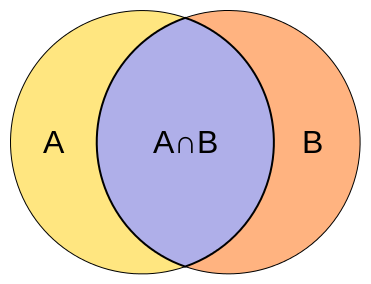
\includegraphics[width=0.23\textwidth]{images/Intersection_of_sets_A_and_B.png} 
    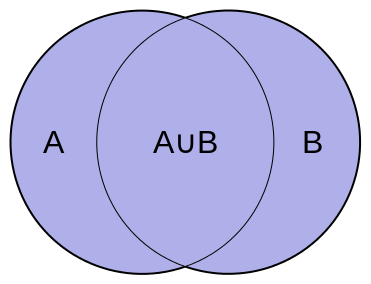
\includegraphics[width=0.23\textwidth]{images/Union_of_sets_A_and_B.png}
    \caption{Intersection and union of two sets $ A $ and $ B $ \cite{intersectionImage,unionImage}}
\end{figure}

The computed Jaccard Coefficient of A and B is  $ J(S_3(A),S_3(B)) = \frac{3}{7} \approx 0.43 $.\\

Calculating the Jaccard Coefficient of two sets and a total number of $ n $ items has a complexity of $ O(n^2) $. For high dimensional sets that contain a lot of items, and therefor have a large $ n $, this is a time consuming task.\\

